% Chapter Template

\chapter{Related Work and Background Theory} % Main chapter title

\label{Chapter2} % Change X to a consecutive number; for referencing this chapter elsewhere, use \ref{ChapterX}
Accurate indoor localization has been examined for a long time. Many different solutions have been developed and presented, using different approaches regarding system architecture and localization method. Within these solutions, mostly client-based architectures can be seen. Moreover, most research focuses on radio-based localization or sensor-based tracking.

In this section, we first give a short overview of the different types of localization systems used in related work. Afterwards we briefly introduce the different system architectures and the different localization techniques. In this second part of the chapter we distinguish between client and server-based system architectures, we introduce fingerprinting-based and range-based localization techniques, as well as the principles of movement detection. The process of information fusion from different data sources and the radio technology of ultra wideband is explained in the last part of this section.

%----------------------------------------------------------------------------------------
%	SECTION 1
%----------------------------------------------------------------------------------------
\section{Overview of Localization System Research}
Localization systems can either be grouped according to their client, server or hybrid architecture or according the type of localization technique they use. The different types of localization techniques are: Fingerprinting, range-based approaches, movement recognition-based or hybrid solutions. 

\subsection{Client-based and Server-based Architecture}
Localization algorithms can either run on a centralized server or on the client device itself. A server-based localization system can be interesting, as it does not require a specific target device hardware, which makes it fairly scalable. Coordination of the different system components and data processing can be done on the server \cite{Delmastro}.
In \cite{Carrera} the system runs on a commodity smartphone, with the benefit of eliminating further communication to an external entity. Such client-based localization systems can often be deployed without any additional hardware when for example WLAN access points are already available. The author's of \cite{Guoguo} use a hybrid of server and client-based architecture - ranges are calculated on the client device while network control and the database are managed on a server. However, their approach strongly relies on high-band acoustic signals, which are highly sensitive to ambient noise and interferences. Furthermore, the long-term exposure of acoustic beacons to humans and animals was not tested, even though some animal species could probably even hear the beacon sound.

%----------------------------------------------------------------------------------------
%	SECTION 2
%----------------------------------------------------------------------------------------
\subsection{Fingerprint Localization}
Fingerprint localization is a range-free localization method, where radio signals and other measurements that are highly affected by environmental conditions are fingerprinted and stored in a map. The position is estimated by comparing a current fingerprint to the existing map. The authors of \cite{Taniuchi} provided a room-based ensemble learning technique for localization. Their room detection uses averaged coordinate outputs of a k-NN estimator. In publication \cite{Carrera2}, the authors propose a discriminative learning method for indoor localization based on a hidden markov model. Their approach is a zone recognition algorithm based on magnetic field and WiFi fingerprints brought together with transition probabilities between zones. Their work only focused on room level localization, which seems like a big restriction for some indoor applications, where localization within a room can be important.

%----------------------------------------------------------------------------------------
%	SECTION 3
%----------------------------------------------------------------------------------------
\subsection{Range-based Localization}
In range-based localization systems, the range is defined as the propagation distance between the target and anchor nodes (AN). First, the propagation distances are calculated. Afterwards, many different algorithms can be used to find the absolute position of the target. In \cite{Horus} a received signal strength indicator is used to estimate the range during the ranging process. A different method to do ranging is used in \cite{IEEE}, where the authors calculated distances by the elapsed time between sending and receiving radio messages. Range-based algorithms are often much lighter and computationally less expensive than fingerprinting methods, as the big effort in generating, storing and processing a radio map falls away. However, only relying on different arrival times of messages can lead to strong influences of environmental conditions, especially non line of sight connections can strongly differ from line of sight connections.

%----------------------------------------------------------------------------------------
%	SECTION 4
%----------------------------------------------------------------------------------------
\subsection{Pedestrian Dead Reckoning}
Pedestrian Dead Reckoning (PDR) relies on inertial measurement unit (IMU) readings to find the new position. PDR systems are often not able to calculate absolute positions, but can calculate the relative change in position. This leads to an accumulation of errors over time, which are in most systems eliminated by adding a different source of information, such as WiFi signals or floorplan information. Different IMU sensor readings are used to obtain a stride length estimation, a heading direction estimation and step recognition. In \cite{Borestein} gyroscope data is used to determine the heading orientation while accelerometer readings provide the displacement. They defined a method called Heuristic Drift Elimination (HDE) to minimize the accumulated errors, by adding a specialized sensor deployed on the foot of the pedestrian. Another method to find the heading direction is used in \cite{Kakiuchi}, where the authors use a kind of digital compass by measuring magnetic field energy. Based on accelerometer readings they classified the movement into a walking and into a running mode. A disadvantage of their strong focus on pedestrians is that these localization techniques cannot easily be adapted for other types of locomotion than walking and running, like driving.  

%----------------------------------------------------------------------------------------
%	SECTION 5
%----------------------------------------------------------------------------------------
\subsection{Hybrid Localization Approaches}
The different characteristics of different types of localization methods make it obvious, that combined localization systems could achieve higher accuracy. In combined approaches, especially relative and absolute measurements are fused to have the advantages of both methods. The authors of \cite{Nagpal} used a fingerprinting-based solution in combination with a digital compass. \cite{Carrera} is a particle filter approach that fuses PDR and radio-based ranging, as well as floorplan information into the localization process. Errors in the PDR system are mitigated by the ranging estimations and vice versa. This makes these approaches highly interesting in the research.\\
\noindent\hspace*{5mm}%
With our hybrid localization system presented in this work, we tried to overcome the different disadvantages by fusing information from various sources, all using already established technologies, such as radio signal transmitting etc. We also kept our system rather unspecific, such that it does not rely on a special type of locomotion or special movement patterns, in order to be usable in many applications.


% Chapter Template


%----------------------------------------------------------------------------------------
%	SECTION 1
%----------------------------------------------------------------------------------------
\section{Client and Server-based Localization}
For many applications, the system architecture is very important. The environmental conditions, the underlying hardware and also dogmatic thoughts are taken into account for real applications to determine the system architecture. There are two main types of system architectures - client-based or server-based - that can be distinguished. However, systems using computational resources of both client and servers are possible, where a clear distinction is no longer possible.\\
\noindent\hspace*{5mm}%
Client-based architectures have the huge advantage that no additional server hardware is needed. The client device collects data used for the localization and processes it to estimate its own position. A client-based localization should be used, when standardized target devices with enough computational power and enough energy supply are localized. As all computations are done on the device itself, no further communication to a seperate server is needed. This ensures that no other application can access the position estimation and it reduces the communication overhead.\\
\noindent\hspace*{5mm}%
A server-based system, however, can be more powerful and computationally complex than client-based systems, as there are no big hardware restrictions. The application itself runs on a centralized server, whereas the client-device is only involved in the data collection process. Therefore the client-hardware does not need much computational power, which allows also to use different, non-standardized devices as a target. Especially when position estimations are not used in applications running on the target device, a server-based architecture is beneficial because of the unlimited server capacity. Often, multiple targets are tracked, which is easily possible with a centralized server approach, as the data of several target devices is directly available on the server and can be further processed. 


%----------------------------------------------------------------------------------------
%	SECTION 2
%----------------------------------------------------------------------------------------
\section{Fingerprinting Localization Technique}
Fingerprinting localization, also known as radio map based technique, uses a dense positioning of anchor nodes in the indoor area of interest. A set of measurements, often received signal strength information (RSSI), serve as a fingerprint at each location. Measurements are not limited to radio signals, other sources such as magnetic field data can also be used. The more unique these measurements are, the better is the localization accuracy. Fingerprinting often consists of an offline phase to generate the radio map and an online phase to retrieve the position with a given fingerprint.\\
\noindent\hspace*{5mm}%
In the offline phase, a radio map is generated with several fingerprints. The radio map can either consist of different fingerprint measurements at given reference points (landmarks) that are used to cover the whole area homogenously, or of fingerprints measured in predefined zones in the area of interest. After this phase, for every location in the grid, a tupel (location, fingerprint) with a unique fingerprint should be available.\\
\noindent\hspace*{5mm}%
The online phase consists of an observed fingerprint at the target's location, on which the localization algorithm can be applied to associate the fingerprint to similar radio map entries. This association is then used to estimate the target's location. The result can either be a concrete position estimation built on the presence of reference points or it can be a probability of the target being in a recognized zone. 

%----------------------------------------------------------------------------------------
%	SECTION 3
%----------------------------------------------------------------------------------------

\section{Range Based Localization}

Range based localization systems depend on an infrastructure in the area of the localization:
\begin{itemize} 
\item \textbf{Target Node (TAG)} is the device that is localized. 
\item \textbf{Anchor Nodes (AN)} are placed on carefully chosen points in the building to encounter the best coverage of the whole area.
\end{itemize}

The key idea of range based positioning is to measure the distance between TAG and ANs. With the use of these distances, the exact position of the TAG can be evaluated using multilateration or similar mathematical models. Several different approaches are possible to determine the distance to an anchor node. They can be classified into two groups. In the one hand, there are algorithms using propagation models, which rely on the reduction in power density of electromagnetic waves propagating through space. On the other hand, algorithms make use of known propagation velocities for radio signals  by measuring the time of flight of transmitted waves. 

%-----------------------------------
%	SUBSECTION 3.1
%-----------------------------------
\subsection{Propagation Models}
An electromagnetic wave loses power when travelling through space. In free space, formula \ref{eqn:freePathLoss} explains the relationship between distance and signal strength \cite{VorlesungCN}:

\begin{equation}
P_{r} = P_{t} (\lambda/4\pi r)^2
\label{eqn:freePathLoss}
\end{equation}

where $P_{r}$ is the received signal strength and $P_{t}$ the transmitted signal strength. $\lambda$ is the wavelength and $r$ the radius, or in other words the distance from the transmitter to the receiver. As this formula is restricted to free-space and often in real indoor environments various kinds of obstacles are present, several other approximations for the relationship between distance and signal power exist. Many indoor positioning algorithms use received signal strength indication (RSSI) to calculate distances to the anchor nodes. RSSI is mainly in use because it can be applied to almost every type of transmitted signal, since RSSI uses universal applicable theory. Two approximations are widely used to take care of the non-free-space environments indoors.\\
\noindent\hspace*{5mm}%
A commonly used model for the relationship of distance and RSS is known as Log-normal Distance Path Loss (LDPL), where the path loss in Decibel (dB) is defined as \cite{Sarkar}:
\begin{equation}
PL = PL_{0} +10 \gamma log_{10} (\frac{d}{d_{0}}) + X_{g}
\label{eqn:LDPL}
\end{equation}

with $\gamma$ as the path loss exponent, $PL_{0}$ a path loss measurement at reference distance $d_0$ and $X_{g}$ a zero-mean Gaussian noise. This generic model can be applied to many different environments. It can even be simplified by defining useful reference distances like done in \cite{Kurt}.\\
\noindent\hspace*{5mm}%
LDPL has shown to be rather inaccurate for indoor environments, which led to a path loss model based on Non-Linear Regression (NLR) as used in \cite{ZanLi}. In this approach, the distance to RSS relationship is modelled with the equation:
\begin{equation}
d_{i} = \alpha_{i} e^{\beta_{i}RSS_{i}}.
\label{eqn:NLR}
\end{equation}
$d_{i}$ is the distance between the $i$-th AN and the TAG, $RSS_{i}$ the measured signal strength at the $i$-th AN and $\alpha_{i}$, $\beta_{i}$ specific coefficients obtained in the area of interest. These two coefficients are rather important for the performance of this approach. They are defined due to extensive calculations based on preliminary measurements as described in \cite{Kurt}.


%-----------------------------------
%	SUBSECTION 3.2
%-----------------------------------
\subsection{Time of Flight Based Models}
A totally different technique to get distance estimations are time of flight based models. Their key idea is that we know the travelling velocity of radio waves, which is approximately the speed of light (\SI{2.99792458e8}{\meter\per\second}). When measuring the time between sending and receiving a radio signal, we can easily convert this time of flight (ToF) to a distance estimation. Time of flights are determined by gathering round-trip times (RTT) in radio signal communication. For accurate RTT results the hardware of transmitter and receiver as well as the operating firmware are very important. For the two presented RTT-measuring techniques, the key characteristics are either a quick responding time or extremely well synchronized sender and receiver.\\
\noindent\hspace*{5mm}%
Two way ranging (TWR) is one of these methods to retrieve an accurate round-trip time. An illustration of the TWR process can be seen in Figure \ref{fig:two_way_ranging}. When operating in TWR mode, the TAG transmits a message to the ANs and registers the exact time of transmission. As soon as the message arrives at its destination, the firmware of the AN instantly captures another timestamp. In an acknowledgement (ACK) message, the timestamp of reception and a timestamp of sending the response is transmitted. When this message arrives at the TAG, again a timestamp is registered. With equation \ref{eqn:TWR}, the time of flight can now be evaluated \cite{SewioTWR}.

\begin{figure}[th]
\centering
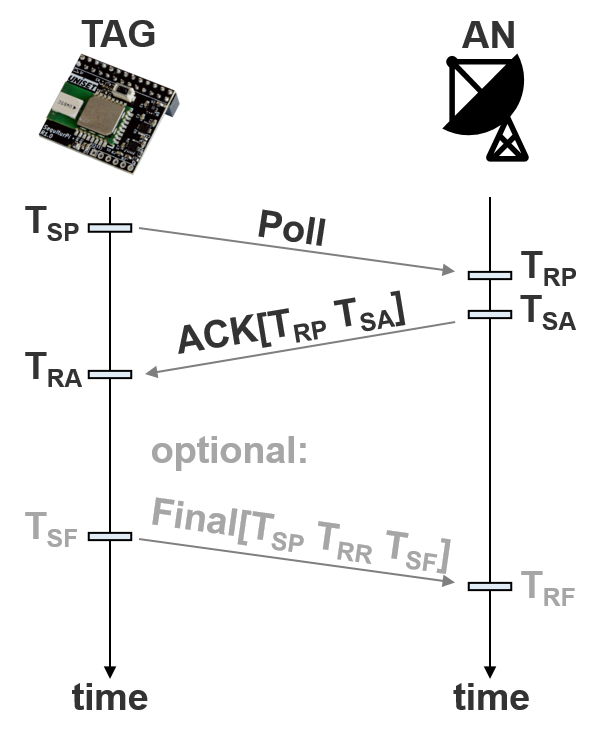
\includegraphics[width=0.5\textwidth]{Figures/two_way_ranging}
\decoRule
\caption[Two Way Ranging]{Illustration of TWR and SDS-TWR communication}
\label{fig:two_way_ranging}
\end{figure}

To achieve higher accuracy, the communication can be extended with a final message containing two additional timestamps of the requester. This is called symmetrical double-sided two-way ranging (SDS-TWR) \cite{Wikipedia} and is indicated as optional in Figure \ref{fig:two_way_ranging}.\\
\\
Evaluation of time of flight for TWR:\\
\begin{equation}
 ToF = [(T_{RA}-T_{SP})-(T_{SA}-T_{RP})] / 2
\label{eqn:TWR}
\end{equation}

Respectively the time of flight for SDS-TWR:\\
\begin{equation}
ToF = [(T_{RA}-T_{SP})-(T_{SA}-T_{RP}) + (T_{RF}-T_{SA})-(T_{SF}-T_{RA}) ]/ 4
\label{eqn:SDS-TWR}
\end{equation}

with the following timestamps, also indicated in Figure \ref{fig:two_way_ranging}: $T_{SP}$ as time of Poll-sending, $T_{RP}$ as time of Poll-reception, $T_{SA}$ as time of ACK-sending, $T_{RA}$ as time of ACK-reception, $T_{SF}$ as time of Final-sending and $T_{RF}$ as time of Final-reception.\\
\noindent\hspace*{5mm}%
A second approach for RTT determination is called time difference of arrival (TDOA). While TWR does not need further synchronization between the devices, TDOA requires very precise synchronization of the anchor nodes. This is normally done by specifying a master node per three to five anchors. For bigger scenarios often multiple dedicated masters are specified. The master nodes transmit repeatedly clock synchronization messages, such that every AN gets at least one sync message. An AN can also receive sync messages from multiple masters. In that case it will store multiple differently synchronized times.
To evaluate the time of flight, a TAG in range will broadcast a blink message. This blink message will initialize the ranging process. Every AN that receives this blink, will capture a timestamp of the time of arrival (or when holding more than one synctime, capture multiple timestamps). These timestamps are forwarded to the server together with a synch ID and a blink transmitter identity. When a server received at least three timestamps with the same synch ID, it can performs the position estimation based on the time of arrival of the initial blink message at each AN.
\begin{figure}[th]
\centering
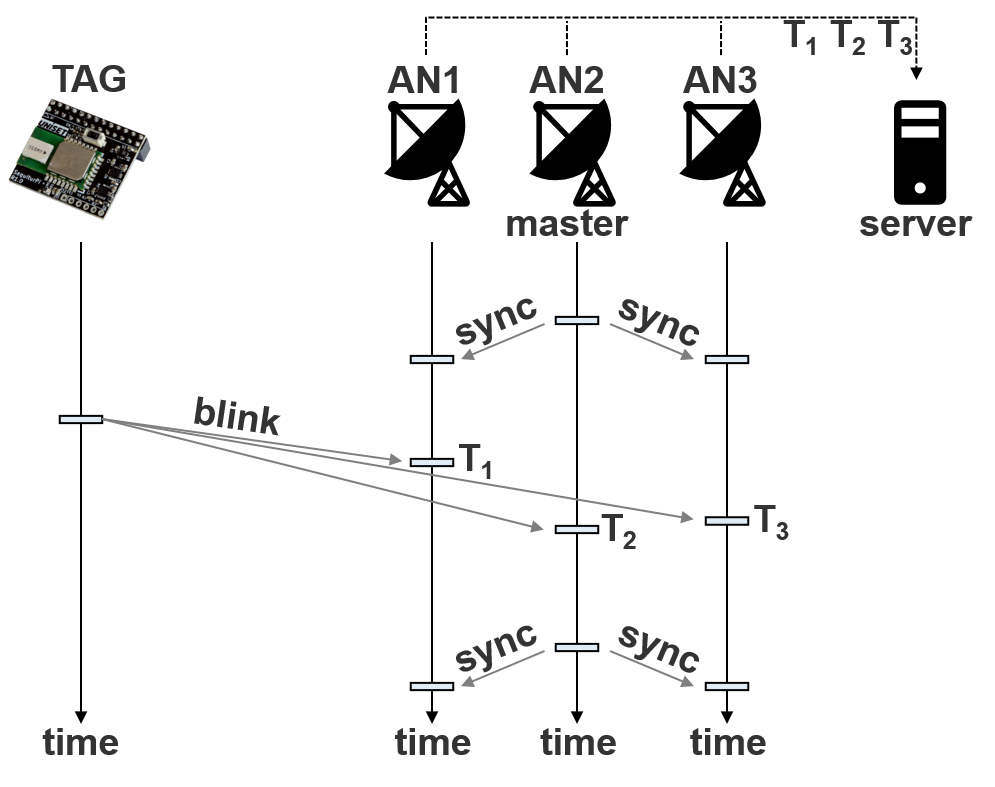
\includegraphics[width=0.7\textwidth]{Figures/time_difference_of_arrival}
\decoRule
\caption[Time Difference of Arrival]{Typical Setup for Time Difference of Arrival communication. Based on \cite{SewioTDOA}.}
\label{fig:time_difference_of_arrival}
\end{figure}
A huge benefit of TDOA is the fact, that the TAG only needs to send one blink message per time interval and will not have to communicate with every AN separately, as in TWR. This can be seen in Figure \ref{fig:time_difference_of_arrival}.\\
\noindent\hspace*{5mm}%
For TWR the overhead grows enormous with every anchor and every TAG that is added. For TDOA hundreds of TAGs can be tracked, with only proportional overhead growth and much lower energy consumption for the TAG.\\
Number of messages sent in one iteration:\\
\\
TWR:  $3 * n_{t} * n_{an}$\\
TDOA:  $n_{t}$\\
where $n_{t}$ is the number of TAGs and $n_{an}$ is the number of anchor nodes \cite{SewioTDOA}.

%-----------------------------------
%	SUBSECTION 3.3
%-----------------------------------
\subsection{Multilateration}
Multilateration is a mathematical method to calculate a position using three or more known values. It is an extension of trilateration, where only three values are used. Triangulation and trilateration use the mathematical concepts of triangles to find unknown lengths. Triangulation was already mentioned by the Greek mathematician Thales, who used this concept for finding out the height of ancient Egypt pyramids \cite{thales}. It was also used for cartography purposes, where angles between fixed points were measured and heights and distances could be calculated. 
Although trilateration and triangulation use the same mathematical triangle concept, the values used in the calculation are different: We call it triangulation, when angles to anchor positions are measured, otherwise - when distances to anchors are measured - it is called trilateration.
As it was easier to measure angles than distances in the past, triangulation was more often used. With modern electronic devices, it is more common to determine distances, rather than angles. 

\begin{figure}[th]
\centering
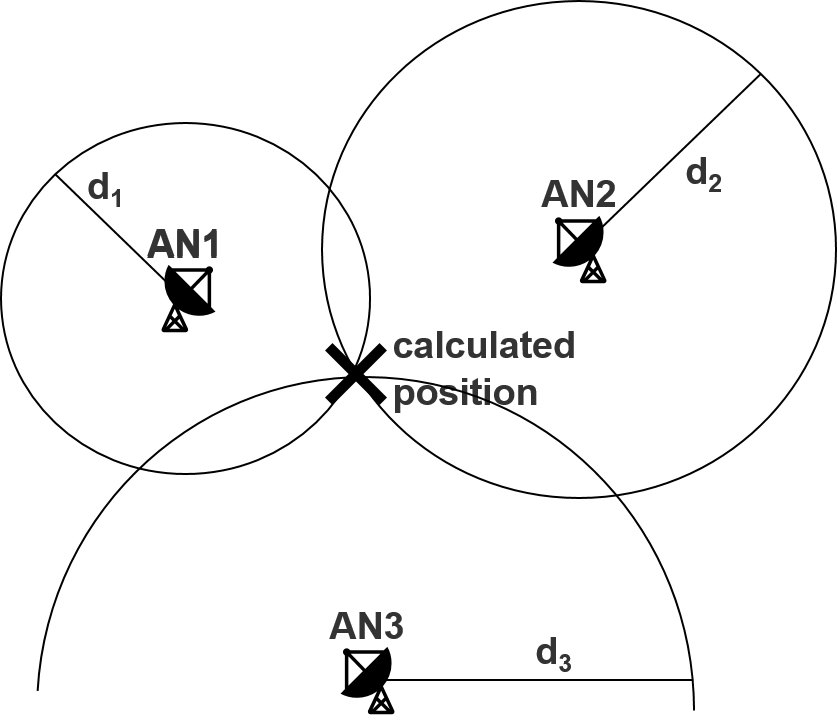
\includegraphics[width=0.6\textwidth]{Figures/trilateration}
\decoRule
\caption[Trilateration]{Graphical illustration of the trilateration concept.}
\label{fig:trilateration}
\end{figure}

Figure \ref{fig:trilateration} shows how trilateration is used for positioning. With the known distance to every AN, a circle with radius of this distance can be drawn around every AN. These circles do only have one common intersection point, that is where the TAG lies. However, this is a theoretical and idealized scenario, where every range can be determined accurately. In real applications, the ranges are not exactly calculated, what leads to the fact that we will not only get a single point for the calculated position, but several points, especially when we use more than three ANs.

%----------------------------------------------------------------------------------------
%	SECTION 4
%----------------------------------------------------------------------------------------
\section{Movement Detection}
Indoor positioning is often reduced to two dimensions, such that the movement vector is also a two-dimensional construct. A movement vector $Mv_{t}$ can be stored as $(X_{t}, Y_{t})$ cartesian coordinates or using a tuple of heading direction angle and stride length $(\theta_{t}, \ell_{t})$. Both, $\theta$ and $\ell$, can be calculated by the IMU readings, where noise occurs such that the heading direction is statistically described as:
\begin{equation}
\theta_{t} = \hat{\theta}_{t} + \theta_{bs,t} + \theta_{be,t} + \epsilon_{\theta, t},
\label{eqn:heading_direction}
\end{equation}
with $\hat{\theta}_{t}$ as the actual heading orientation,  $\theta_{bs,t}$ as a sensor bias introduced by uncalibrated sensor readings, $\theta_{be,t}$ as an environmental angular bias due to magnetic field disturbances and $\epsilon_{\theta, t}$ as a measured random error. The heading direction can be calculated by using the geomagnetic field of the earth. The formula $\theta = atan(\frac{mag_{x}}{mag_{y}})$ can be used to obtain the heading direction, where $mag_{x}$ and $mag_{y}$ are the magnetic field sensor readings in X direction, respectively in Y direction.\\
\noindent\hspace*{5mm}%
Whereas the heading direction is obtained by measuring absolute values of magnetic field energy, the accelerometer data is a relative quantity that is used for stride length determination. Dealing with relative values, measured errors propagate over time. So it is almost impossible to use relative quantities (e.g. acceleration) to calculate absolute quantities (e.g. distance) over a longer period of time. To address this, an absolute quantity is needed to correct long-term errors. Velocities from previous time slots can be used for this. As we can not assume the acceleration to be constant during a whole time slot, the movement length approximation can be defined as: 
\begin{equation}
\ell_{t} = \hat{\ell}_{t-1} + \sum_{i=0}^{N}([(\hat{a}_{i} + a_{bs,i} +\epsilon_{a, i}) * \Delta t_{i} ]*(N-i)) *\Delta t + \epsilon_{\ell, t},
\label{eqn:stride_length}
\end{equation}
where $\hat{\ell}_{t-1}$ is the actual movement length of time period $t-1$, $\hat{a}_{i}$ is the actual middle acceleration during the $i$-th of N time slots in time period $\Delta t$, $a_{bs,i}$ is another sensor bias due to uncalibrated sensor readings and $\epsilon_{a, i}$ as well as $\epsilon_{\ell, t}$ are measured random errors in acceleration and distance respectively.


%----------------------------------------------------------------------------------------
%	SECTION 5
%----------------------------------------------------------------------------------------

\section{Data Fusion for Localization}
When several different sources of data are collected and brought together in one algorithm, we call it data fusion. There are several common ways of fusing data, the most widely used are filtering approaches such as the Kalman Filter \cite{Kurt} and the Particle Filter \cite{Carrera}. The focus of this work lies on a particle filter approach, also known as Monte Carlo Localization (MCL), which is often used for indoor positioning. It combines various noisy measurements to estimate the system state and minimize errors. To introduce the particle filter, we explain its three main phases and the corresponding inputs. 

\subsection{Particle Filter: Prediction Phase}
In the prediction phase, every particle is repositioned. At time $t$, each particle has a state vector that is defined as follows:
\begin{equation}
X_{t} = [x_{t}, y_{t}, x_{t-1}, y_{t-1}],
\label{eqn:particles}
\end{equation}
where $(x_{t}, y_{t})$ corresponds to the Cartesian coordinates of the particle at time $t$ and $(x_{t-1}, y_{t-1})$ at time $t-1$ respectively. The repositioning of the particles is often done randomly. However, it could also be done according to the movement vector or other sensor-based values. If present, floorplan restrictions are applied in this phase, whereas movements through walls are not permitted, they lead to another prediction iteration for that particle.

\subsection{Particle Filter: Observation Phase}
In the observation phase, the associated particle weight $w^{i}_{t}$ is recalculated for every particle since the weight does not anymore correspond to the current position. For each anchor node, we have an obtained distance measurement $d^{j}_{t}$, which itself contains various errors. Statistically, it can be described as: 
\begin{equation}
d^{j}_{t} = \hat{d}^{j}_{t} + d^{j}_{be, t} + \epsilon_{d^{j}, t},
\label{eqn:distances}
\end{equation}
where $\hat{d}^{j}_{t}$ is the actual distance to node $j$, $d^{j}_{be, t}$ is an environmental bias due to local conditions and $\epsilon_{d^{j}, t},$ is a measured random error.\\
\noindent\hspace*{5mm}%
With the given observation vector $Zd_{t} = [d_{t}^{j}], j = 1...N$, at time $t$, where $N$ is the number of
ANs, the weight of each particle can be recalculated. Each particle's weight is updated corresponding to the likelihood of the range observations conditioned on each particle $p(Zd_{t} | X^{i}_{t})$ at time t, and the likelihood of the motion observation conditioned on each particle $p(Mv_{t} | X^{i}_{t})$ at time t respectively.


 Then, the probabilities are determined as:
\begin{equation}
p(Zd_{t} | X^{i}_{t}) = p(d_{t}^{j} | X^{i}_{t})
\label{eqn:probability_distance}
\end{equation}
and
\begin{equation}
p(Mv_{t} | X^{i}_{t}) = p(M_{x,t} | X^{i}_{t}) * p(M_{y,t} | X^{i}_{t}).
\label{eqn:probability_movement}
\end{equation}
In addition, the zone probability is:
\begin{equation}
p(y_t | X^{i}_{t}) = p_{tot}(y_{t} | z^{i}_{t}),
\label{eqn:probability_zone}
\end{equation}
where $y_t$ is the observed fingerprint at time $t$ and $z^{i}_{t}$ the current zone of particle $X^{i}$.
In order to avoid confusion between different likelihoods used in this work, hereafter we refer to $p(d_{t} | X^{i}_{t})$ as the ranging likelihood, $p(M_{t} | X^{i}_{t})$ for the motion likelihood, $p(y_t | X^{i}_{t})$ for the zone likelihood and $p(Z_{t} | X^{i}_{t})$ as the overall likelihood.

The associated weight $w^{i}_{t}$ of each particle is given by range as well as by motion information. A particle at the current position $(x_{t},y_{t})$ with low probability to observe $d_{t}^{j}$ in its position will be assigned a small weight. Additionally, a particle that moved in x-direction by $x_{t}^{i}-x_{t-1}^{i}$ with low probability to observe the movement $M_{x,t}$ will also be assigned a small weight. The same principle is used to update the weight according to the movement in y-direction.
That leads to the fact that particles with large weights will have a stronger effect on the determination of the state of the system.
We assume that all these likelihoods - the ranges to each AN as well as the movement in direction x, y - are statistically independent of each other. Therefore, the overall likelihood is defined as:
\begin{equation}
p(Z_{t} | X^{i}_{t}) = \prod_{j=1}^{N} p(\hat{d}_{j,t}|X_{t}^{i}) * p(\hat{M}_{x,t} | X^{i}_{t}) * p(\hat{M}_{y,t} | X^{i}_{t}) * p(y_t | X^{i}_{t}),
\label{eqn:probability_overall}
\end{equation}
where $\hat{d}_{j,t}$ is the measured distance to the AN j at time t and $\hat{M}_{x,t}$ is the measured motion in x-direction in timeinterval t, respectively $\hat{M}_{y,t}$ in y-direction and $y_t$ is the measured RSS fingerprint.

The individual likelihood for the range observation can then be expressed as:
\begin{equation}
p(\hat{d}_{j,t} | X^{i}_{t}) = \frac{1}{\sqrt{2\pi \sigma_{j}^{2}}} * exp(\frac{-[\sqrt{(x^{i}_{t}-x_{j})^{2}+(y^{i}_{t}-y_{j})^{2}} - \hat{d}_{j,t}]^{2}}{2\sigma_{j}^{2}}),
\label{eqn:probability_individual_distance}
\end{equation}
where $(x_{j},y_{j})$ are the known coordinates of the $j$-th AN.
Finally, the individual likelihood of the motion observation in x-direction (analogue for y-direction) is expressed as follows:

\begin{equation}
p(\hat{M}_{x,t} | X^{i}_{t}) = \frac{1}{2\pi \sigma_{Mx}^{2}} * exp(\frac{-[(x^{i}_{t}-x^{i}_{t-1}) - \hat{M}_{x,t}]^{2}}{2\sigma_{Mx}^{2}})
\label{eqn:probability_individual_movement}
\end{equation}

\subsection{Particle Filter: Resampling Phase}
The resampling phase is an essential component of a particle filter implementation, although it is a computationally expensive step. In the resampling, particles with low assigned weights are repositioned at identical positions as particles with high associated weights. This means that after the repositioning of the prediction phase and after the weight calculation in the observation phase, a resampling in a systematic manner is done. This resampling relies on the overall likelihood $p(Z_{t} | X^{i}_{t})$, which means that every kind of likelihood is taken into account for this step. After repositioning the particles with low weights (and after updating their weight), all weights are normalized to obtain in the next step the weighted center of all particles, which corresponds to the estimated position. 

%----------------------------------------------------------------------------------------
%	SECTION 6
%----------------------------------------------------------------------------------------


\section{Ultra Wideband Radio Technology}
Ultra wide-band (UWB) is a radio technology in use for military and industrial communication, positioning and collecting sensor data. Unlike other communication technologies, UWB occupies a wide area of frequencies instead of just covering a small frequency spectrum. As shown in Figure \ref{fig:frequency_spectrum}, UWB spans over a spectrum of more than 500 megahertz (MHz) that lies within the range of 3.1 gigahertz (GHz) and 13.6 GHz.
\begin{figure}[th]
\centering
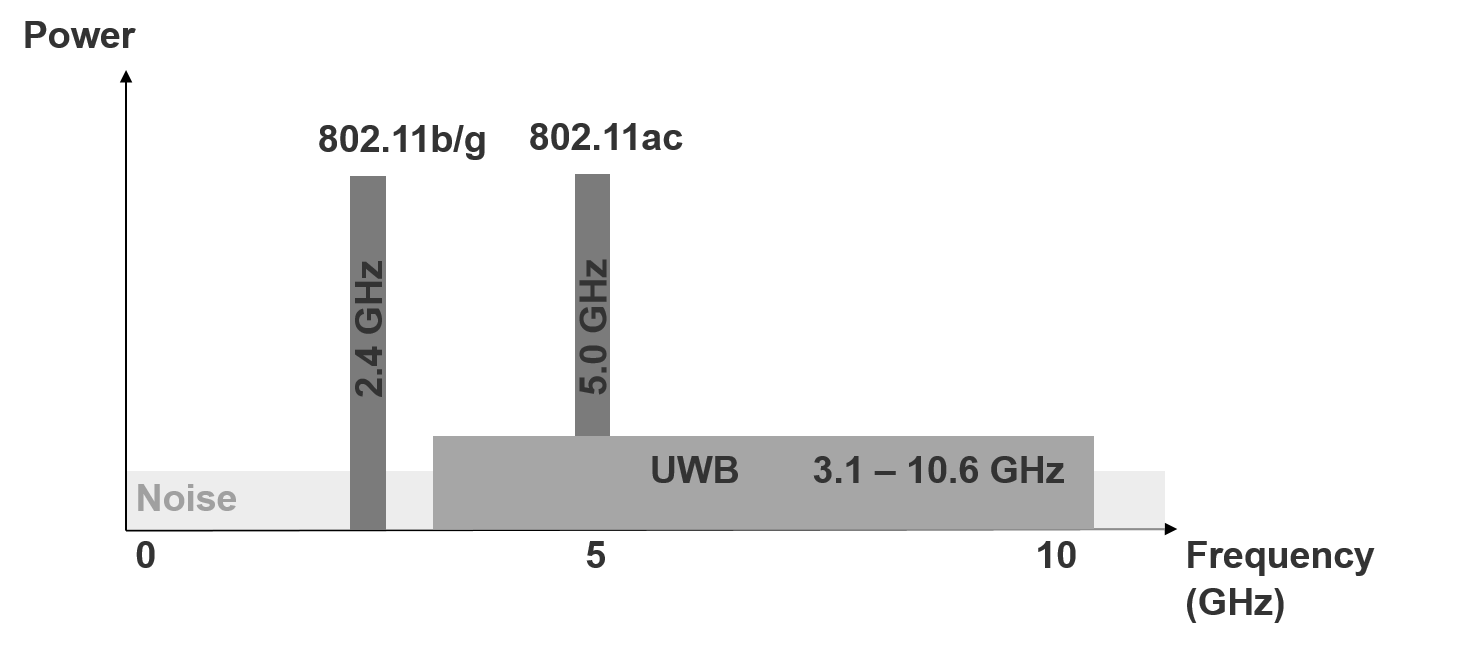
\includegraphics[width=1.0\textwidth]{Figures/frequency_spectrum}
\decoRule
\caption[UWB Frequency Spectrum]{Comparison of Wi-Fi (802.11) and UWB frequencies.}
\label{fig:frequency_spectrum}
\end{figure}
UWB operates with less energy compared to other communication like Wi-Fi. However, the main difference between UWB and conventional radio transmissions is the underlying modulation technique. UWB transmits data by generating extremely short radio energy pulses at specific times instead of varying frequency and phase of sinus waves. In addition to the pulse position, the pulses can carry information either by their polarity, their amplitude or by using orthogonal pulses.
A single pulse is kept as short as possible, such that more than 100 million, sometimes even continuous streams with more than 1 billion pulses per second, are generated. As single pulses can be registered and identified by the receiver, UWB devices are able to determine very exact ToFs such that distance estimations can be done to high resolution.\\
\noindent\hspace*{5mm}%
The pulse rate highly influences the transmission rate of an UWB communication. The pulse frequency varies between 1 million pulses per second to over 1 billion pulses. Devices often support different operation modes, such that the number of pulses can be configured. However, with a higher pulse rate, the transmitting distance decreases, such that a trade-off between data rate and communication distance occurs. In Table \ref{tab:pulse_rate_range} the approximate correlation between pulse rate, bit rate and range is shown \cite{ITU}. In a cluttered environment, especially for non-line of sight communications, the possible communication distance decreases very fast. This has to be considered for indoor applications, as line of sight is very rare in an indoor scenario.

\begin{table}
\caption{Relationship of Pulse Rates and Communication Distance}
\label{tab:pulse_rate_range}
\centering
\begin{tabular}{c c c}
\toprule
\textbf{Pulse rate}[pulse/s] & \textbf{Bit rate}[Mbit/s] & \textbf{Range}[m]\\
\midrule
1'000'000 & \textasciitilde40 & \textasciitilde100\\
500'000'000 & \textasciitilde100 & \textasciitilde10\\
1'000'000'000 & \textasciitilde500 & 4-10\\
\bottomrule\\
\end{tabular}
\end{table}